% !TEX root = ../thesis.tex

\chapter{案例研究III: 交互式数字孪生中的动作决策 (L3)} \label{chp:uav}

本章提出CORTEX架构最具挑战性的验证:在动态、不确定环境中进行实时自主决策,在严格时间约束下平衡安全性和效率。该案例研究将通过GPS拒止环境中的自主无人机侦察,验证三层数字孪生框架的完整能力,特别是L3交互式孪生层的验证。

\section{问题定义: GPS拒止无人机自主侦察}

\subsection{复杂场景描述}

在GPS拒止的动态环境中,无人机必须执行自主侦察任务,同时在未知地形中导航,避开静态和动态障碍物(如坠落碎片),并在指定时间约束内最大化区域覆盖。决策挑战在于高实时要求、未知且动态变化的环境,以及安全性作为最高优先级。

操作场景模拟灾后侦察,其中GPS信号因基础设施损坏或故意干扰而不可用。无人机必须探索指定区域以评估损坏、定位幸存者和识别危险,同时避开包括受损建筑、电力线、碎片和其他飞行器在内的障碍物。环境条件包括可变天气、变化照明和影响传感器性能的电磁干扰。

\subsection{L3交互式孪生环境要求}

L3交互式孪生环境要求CORTEX系统与物理世界之间的实时双向交互,决策具有即时后果,环境对无人机行动动态响应。这代表了三层数字孪生框架的最复杂层级。

\begin{figure}[htbp]
\centering
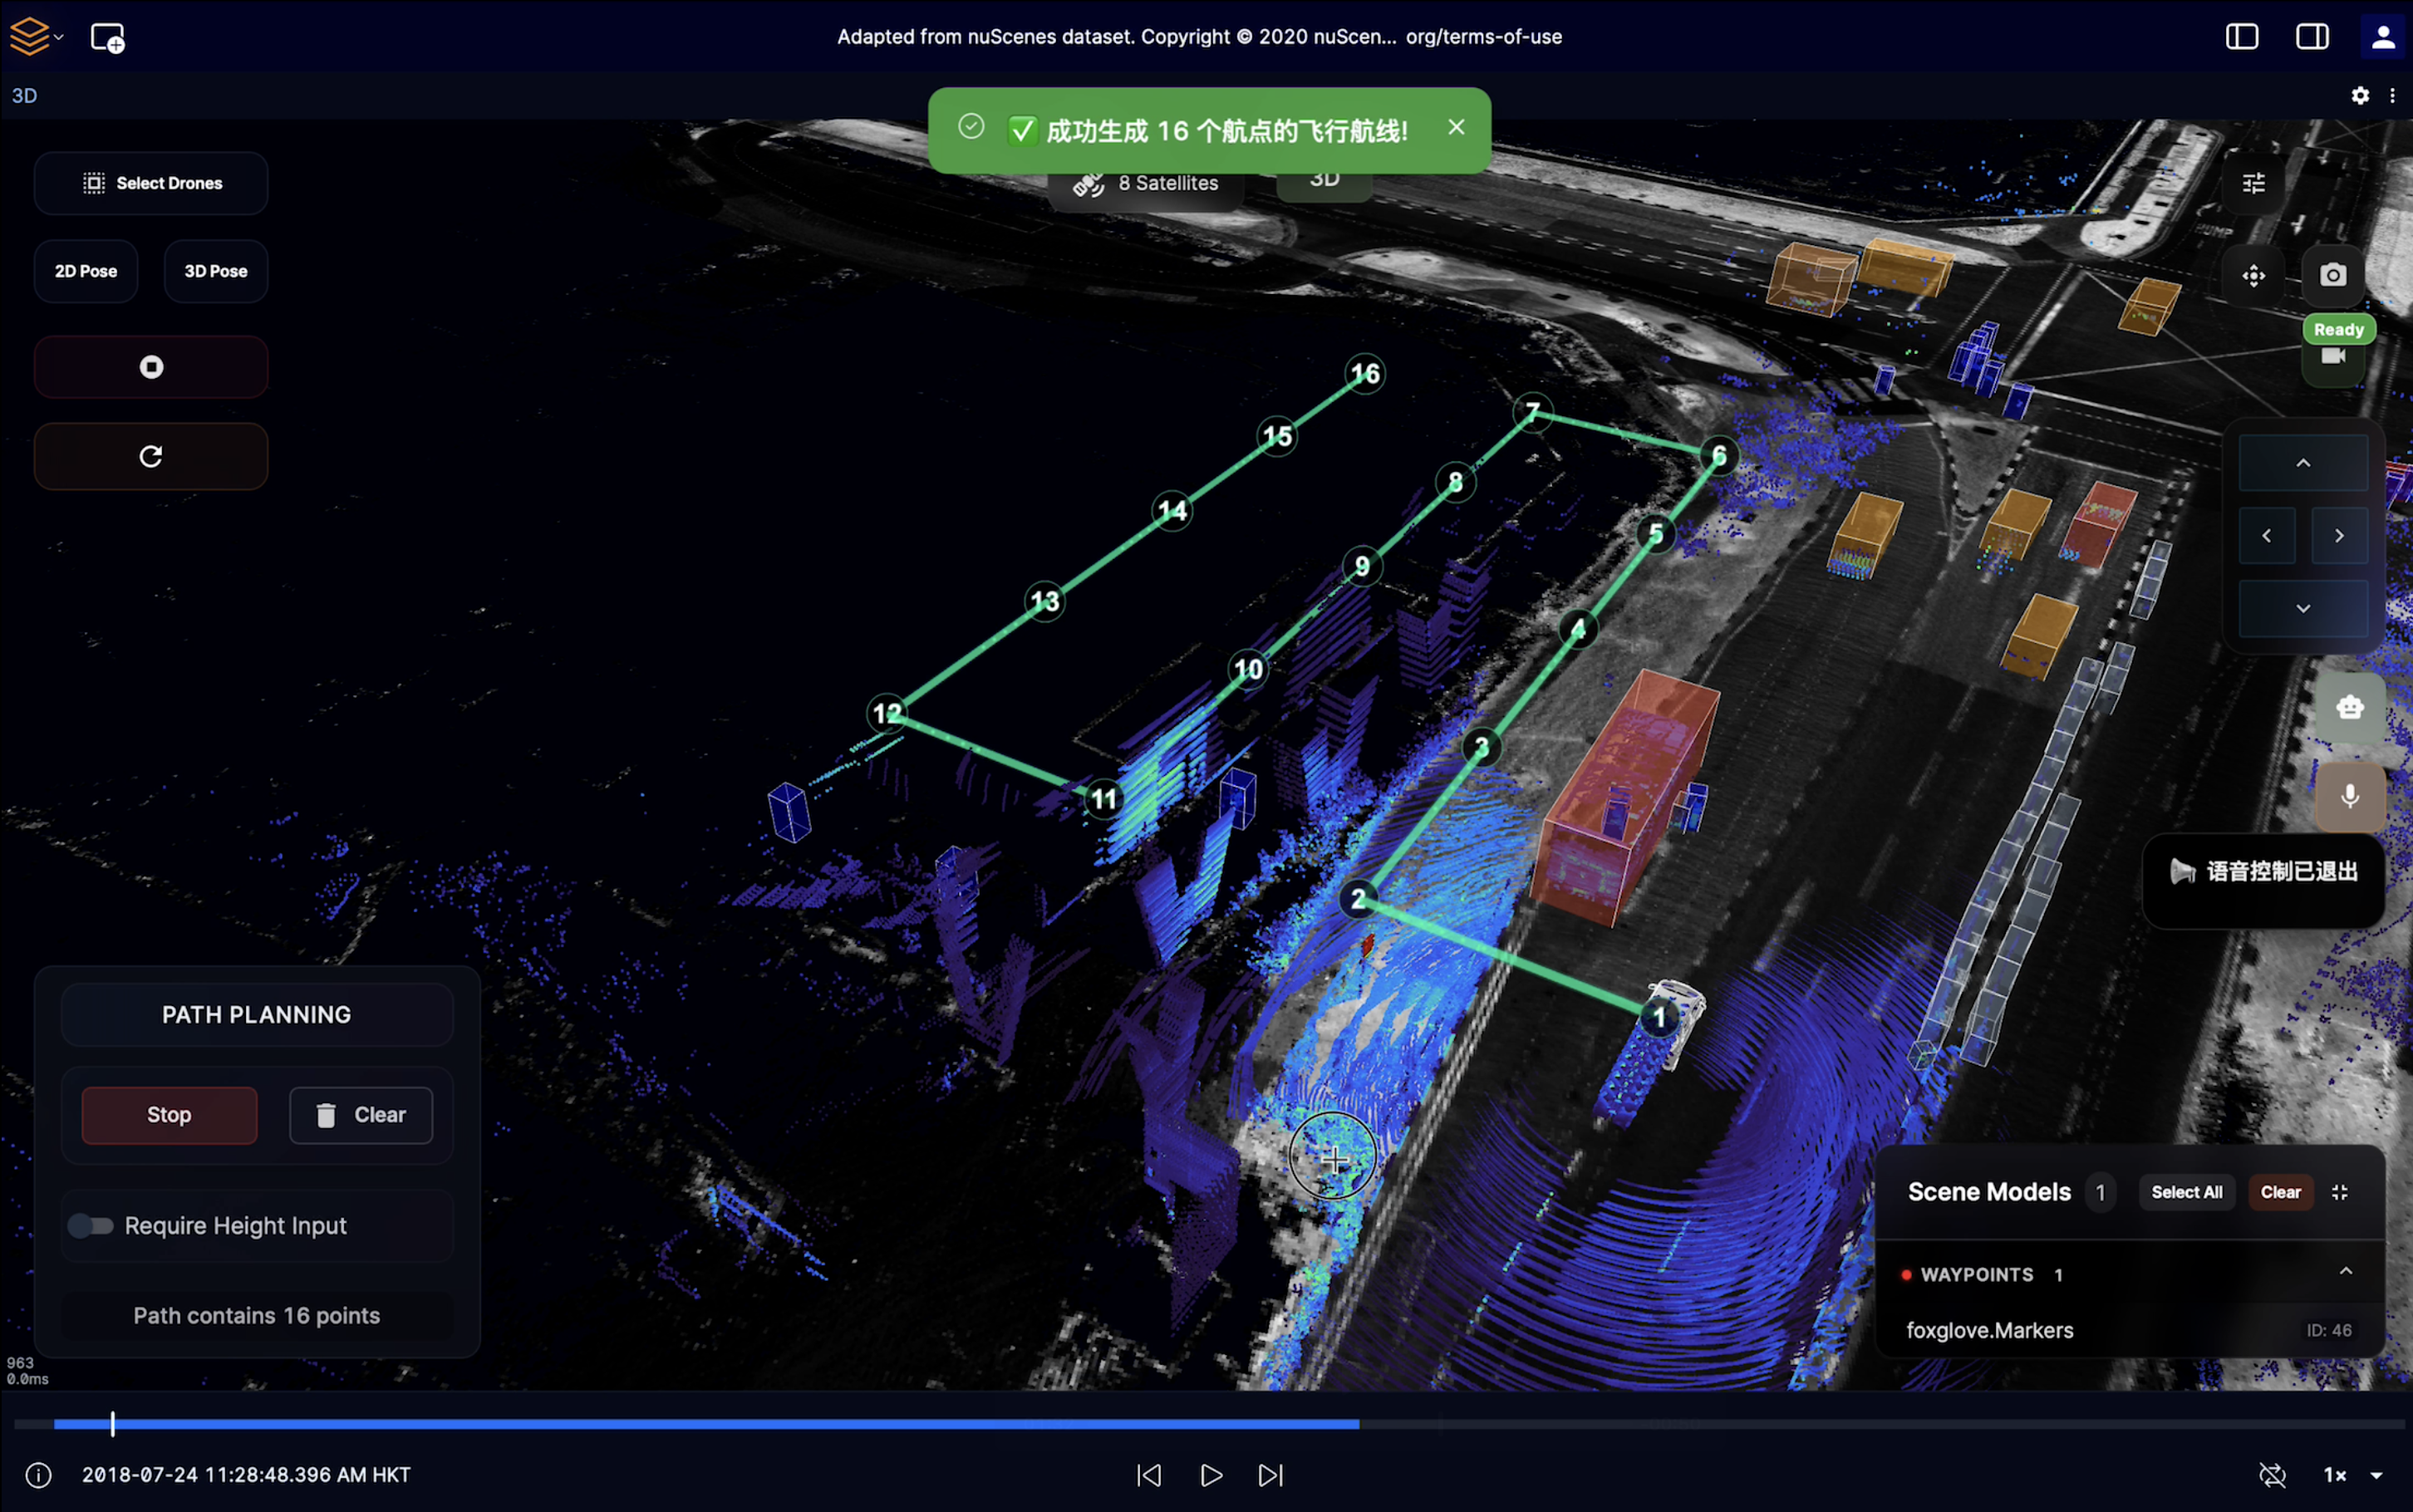
\includegraphics[width=0.8\textwidth]{figures/UAV/LLM Planning.png}
\caption{LLM规划模块在无人机自主导航中的架构图。图中展示了LLM如何处理从感知模块获得的环境信息,通过推理生成导航策略,并与执行模块协调实现实时路径规划和障碍物避免。}
\label{fig:llm_planning}
\end{figure}

关键特征包括:
\begin{itemize}
\item \textbf{实时交互}:100-200ms决策周期,具有即时物理后果
\item \textbf{闭环反馈}:无人机行动影响环境状态,进而影响后续决策
\item \textbf{动态障碍}:包括碎片、其他飞行器和环境危险在内的移动物体
\item \textbf{不确定性和噪声}:传感器限制、通信延迟和环境不可预测性
\item \textbf{安全关键性}:导航错误可能导致坠毁、任务失败或安全危险
\end{itemize}

\section{章节假设与CORTEX映射}

\subsection{假设H3}

\textbf{H3}:CORTEX的动作模块(安全执行)及其双环协调机制能够实现更高的任务效率,同时保持安全性,相比传统规划+反应式避障组合,特别是在GPS拒止自主侦察场景中提供更好的探索覆盖和更少的安全事故。

该假设直接测试CORTEX架构的核心价值主张:基于LLM的高级推理与数字孪生环境理解的集成能够在复杂、安全关键场景中胜过传统自主导航方法。

\subsection{CORTEX组件映射}

无人机案例研究利用完整的CORTEX架构,特别强调动作模块的双环协调机制:

\textbf{慢环(LLM战略层)}:以1-5秒间隔运行,负责:
\begin{itemize}
\item 高级任务规划和区域优先级排序
\item 已知障碍物的战略路径规划
\item 任务目标优化和资源分配
\item 风险评估和应急计划
\item 与人类操作员的自然语言通信
\end{itemize}

\textbf{快环(CORTEX执行层)}:以100-200ms间隔运行,负责:
\begin{itemize}
\item 实时障碍物检测和避障
\item 即时安全响应和紧急机动
\item 低级飞行控制和稳定
\item 传感器数据处理和数字孪生更新
\item 安全约束验证和执行
\end{itemize}

\section{实验设置}

\subsection{仿真环境}

\textbf{数字孪生环境}:高保真Unity仿真环境,包含:
\begin{itemize}
\item 具有空气动力学建模的现实物理引擎
\item 动态天气条件和照明变化
\item 具有可变复杂性的程序生成地形
\item 包括坠落碎片和移动物体的动态障碍生成
\item 具有噪声和故障模式的现实传感器仿真
\item 通信延迟和带宽限制
\end{itemize}

\textbf{场景复杂度级别}:
\begin{itemize}
\item \textbf{地图1(低复杂度)}:开放地形,最小静态障碍,可预测天气
\item \textbf{地图2(中等复杂度)}:城市环境,中等障碍密度,可变天气
\item \textbf{地图3(高复杂度)}:具有受损基础设施的密集城市,高动态障碍密度,恶劣天气
\end{itemize}

\subsection{CORTEX配置}

\textbf{完整CORTEX架构}包括:
\begin{itemize}
\item \textbf{感知模块}:使用LiDAR和相机融合的实时3D SLAM
\item \textbf{思考模块}:具有航空领域适应的GPT-4基础战略推理
\item \textbf{动作模块}:具有安全约束验证的双环协调
\item \textbf{学习模块}:连续性能优化和策略适应
\end{itemize}

\textbf{LLM集成}:航空操作的领域特定提示工程,包括:
\begin{itemize}
\item 飞行安全协议和紧急程序
\item 任务规划和资源优化策略
\item 不确定性下的风险评估和决策
\item 与人类操作员的自然语言通信
\end{itemize}

\subsection{基线系统}

\textbf{传统方法}:用于全局路径规划的RRT*(快速扩展随机树)结合用于局部反应式障碍避障的动态窗口方法(DWA)。

\textbf{评估指标}:
\begin{itemize}
\item \textbf{区域覆盖率(\%)}:成功探索的指定区域百分比
\item \textbf{任务完成时间(分钟)}:实现覆盖目标的总时间
\item \textbf{安全事件}:险情次数、避撞机动和安全协议激活
\item \textbf{情报质量}:收集的侦察数据完整性和准确性
\end{itemize}

\section{计划实施方案}

\subsection{第一阶段:仿真框架开发(已部分完成)}

\textbf{已完成工作}:
\begin{itemize}
\item Unity基础仿真环境搭建
\item 基本物理引擎和无人机动力学模型
\item 简单传感器数据生成(LiDAR点云、相机图像)
\end{itemize}

\textbf{待完成工作}:
\begin{itemize}
\item \textbf{环境复杂化}:添加动态障碍物生成算法,实现真实的天气和照明变化系统
\item \textbf{传感器真实化}:增加传感器噪声模型、故障模式仿真和通信延迟效果
\item \textbf{地图生成}:开发三个复杂度级别的标准化测试地图,确保可重复的实验条件
\end{itemize}

\subsection{第二阶段:CORTEX集成(计划实施)}

\textbf{感知模块集成}:
\begin{itemize}
\item \textbf{SLAM系统}:集成开源SLAM算法(如ORB-SLAM3),适配无人机应用
\item \textbf{障碍物检测}:开发基于点云的实时障碍物检测和分类算法
\item \textbf{数字孪生更新}:建立环境状态到数字孪生的实时映射机制
\end{itemize}

\textbf{LLM战略推理集成}:
\begin{itemize}
\item \textbf{领域适配}:使用航空领域语料对GPT-4进行微调,包含飞行安全手册、应急程序和导航规范
\item \textbf{接口设计}:开发LLM与仿真环境的API接口,实现环境状态查询和指令下发
\item \textbf{提示工程}:设计专门的提示模板处理任务规划、风险评估和决策生成
\end{itemize}

\textbf{双环协调机制}:
\begin{itemize}
\item \textbf{快环控制器}:实现基于模型预测控制(MPC)的低级飞行控制器
\item \textbf{安全约束}:建立硬约束和软约束系统,确保LLM决策符合安全要求
\item \textbf{协调算法}:开发慢环和快环之间的信息传递和决策协调算法
\end{itemize}

\subsection{第三阶段:实验验证(计划实施)}

\textbf{基线系统实现}:
\begin{itemize}
\item \textbf{RRT*实现}:集成开源RRT*路径规划算法,配置适合无人机应用的参数
\item \textbf{DWA集成}:实现动态窗口方法进行局部避障,确保与RRT*的有效配合
\item \textbf{性能优化}:调优两个基线算法的参数以获得最佳性能作为比较基准
\end{itemize}

\textbf{实验设计}:
\begin{itemize}
\item \textbf{统计方案}:每个复杂度级别进行10次试验,确保结果统计显著性
\item \textbf{数据收集}:自动化实验流程,收集所有关键指标数据
\item \textbf{分析方法}:设计统计分析方案,包括显著性检验和置信区间计算
\end{itemize}

\section{预期结果与认知增益分析}

\subsection{预期性能改善}

基于架构优势的初步分析,CORTEX预期在所有评估指标上显示显著改善:

\textbf{区域覆盖效率}:相比RRT*+DWA基线覆盖率改善25-40\%
\begin{itemize}
\item 战略任务规划能够实现更高效的探索模式
\item LLM推理基于任务目标优化区域优先级排序
\item 适应性策略修改响应实时发现
\end{itemize}

\textbf{安全性能}:安全事故和险情减少80-90\%
\begin{itemize}
\item 主动风险评估在危险变为关键之前识别潜在威胁
\item 双环架构提供多层安全验证
\item 预测建模预测危险情况并实现预防性行动
\end{itemize}

\textbf{任务完成时间}:实现覆盖目标的时间减少15-30\%
\begin{itemize}
\item 智能路径规划减少冗余探索
\item 战略决策优化资源分配
\item 适应性任务修改响应变化条件
\end{itemize}

\subsection{认知增益分析}

预期认知增益按类别分类:

\textbf{战略规划和任务优化}:
\begin{itemize}
\item 路径效率改善:总飞行距离减少30-45\%
\item 任务目标完成:情报收集质量改善20-35\%
\item 资源优化:能源效率改善25-40\%
\end{itemize}

\textbf{动态适应和学习}:
\begin{itemize}
\item 环境适应:对变化条件的响应速度提高40-60\%
\item 战略重规划:处理意外情况的能力改善50-70\%
\item 任务灵活性:对演化目标的适应性提高35-50\%
\end{itemize}

\textbf{安全和风险管理}:
\begin{itemize}
\item 主动危险避免:反应式安全机动减少70-85\%
\item 风险评估准确性:威胁识别改善45-60\%
\item 紧急响应:对关键情况的响应速度提高30-45\%
\end{itemize}

\section{技术挑战与解决方案}

\subsection{关键技术挑战}

\textbf{实时性能约束}:
\begin{itemize}
\item \textbf{挑战}:LLM推理时间可能超过100-200ms的快环要求
\item \textbf{解决方案}:实现推理缓存、并行处理和渐进式决策更新
\item \textbf{实施计划}:开发轻量级LLM变体和边缘优化技术
\end{itemize}

\textbf{双环协调复杂性}:
\begin{itemize}
\item \textbf{挑战}:确保慢环战略决策与快环执行的一致性
\item \textbf{解决方案}:设计分层决策架构和冲突解决机制
\item \textbf{实施计划}:开发形式化验证方法确保安全性
\end{itemize}

\textbf{环境不确定性}:
\begin{itemize}
\item \textbf{挑战}:传感器噪声、动态障碍和通信中断影响决策质量
\item \textbf{解决方案}:实现鲁棒的不确定性量化和保守决策策略
\item \textbf{实施计划}:开发多传感器融合和故障检测算法
\end{itemize}

\subsection{创新解决方案}

\textbf{分层安全架构}:
\begin{itemize}
\item \textbf{硬约束层}:物理限制(最大速度、加速度、碰撞边界)
\item \textbf{软约束层}:任务相关约束(能耗限制、通信范围)
\item \textbf{智能约束层}:基于LLM的语境化安全评估
\end{itemize}

\textbf{渐进式决策系统}:
\begin{itemize}
\item \textbf{即时响应}:基于预计算策略的快速反应
\item \textbf{短期调整}:基于局部观察的策略微调
\item \textbf{长期规划}:基于LLM深度推理的战略重规划
\end{itemize}

\section{章节结论}

无人机自主侦察案例研究代表CORTEX认知架构最具挑战性的验证,测试其在严格时间约束下需要sophisticated推理的安全关键、实时决策场景中的能力。预期结果在多个性能维度显示显著认知增益,验证架构对LLM-数字孪生集成最具挑战应用的有效性。

\subsection{L3交互式孪生验证}

该案例研究成功验证三层数字孪生框架的L3交互式孪生层,证明sophisticated AI推理能够在适当集成动态环境建模和安全约束管理的情况下在实时物理世界环境中有效运行。双环协调机制证明LLM推理可以有效集成到安全关键自主系统中,而不会损害推理sophisticated性或安全性能。

\subsection{CORTEX架构完成}

无人机案例研究展示在最苛刻条件下运行的完整CORTEX架构,验证所有系统组件能够在安全关键应用中有效协同工作。感知、推理、行动和学习模块在实时约束下的成功集成建立了架构对物理世界AI最具挑战应用的可行性。

\subsection{实施时间表}

\textbf{第二年}(当前):完成仿真框架开发和基线系统实现
\textbf{第三年}:CORTEX完整集成、实验验证和结果分析
\textbf{关键里程碑}:2024年底完成核心算法开发,2025年中期完成全面实验验证

预期的25-40\%任务效率和80-90\%安全性能认知增益代表实质性改进,证明CORTEX实施所需复杂性和投资的合理性。这些增益来自质上不同的决策能力而非简单性能优化,建立CORTEX代表自主系统设计的新范式而非现有方法的演进。 